%%% MA-Chunk, AAMAS 2027 submission.
%%% Tables in generated/ and figures in figs/ are produced by the scripts in scripts/paper/ of the code release.
%%%%%%%%%%%%%%%%%%%%%%%%%%%%%%%%%%%%%%%%%%%%%%%%%%%%%%%%%%%%%%%%%%%%%%%%

%%% LaTeX Template for AAMAS-2027 (based on sigconf.tex)
%%% Prepared by the AAMAS-2027 Publication Chairs based on the version from AAMAS-2026. 

%%%%%%%%%%%%%%%%%%%%%%%%%%%%%%%%%%%%%%%%%%%%%%%%%%%%%%%%%%%%%%%%%%%%%%%%

%%% Start your document with the \documentclass command.


%%% == IMPORTANT ==
%%% Use the first variant below to anonymize your submission (no author information shown).
%%% Use the second variant below for the final paper (including author information).
%%% For further information on anonymity and double-blind reviewing, 
%%% please consult the call for paper information
%%% https://warwick.ac.uk/fac/sci/dcs/aamas2027/calls/

%%%% For anonymized submission, use this
\documentclass[sigconf,anonymous]{aamas} 

%%%% For camera-ready, use this
%\documentclass[sigconf]{aamas} 


%%% Load required packages here (note that many are included already).

\usepackage{balance} % for balancing columns on the final page
\usepackage{multirow}

%%%%%%%%%%%%%%%%%%%%%%%%%%%%%%%%%%%%%%%%%%%%%%%%%%%%%%%%%%%%%%%%%%%%%%%%

%%% AAMAS-2027 copyright block (do not change!)

\makeatletter
\gdef\@copyrightpermission{
  \begin{minipage}{0.2\columnwidth}
   \href{https://creativecommons.org/licenses/by/4.0/}{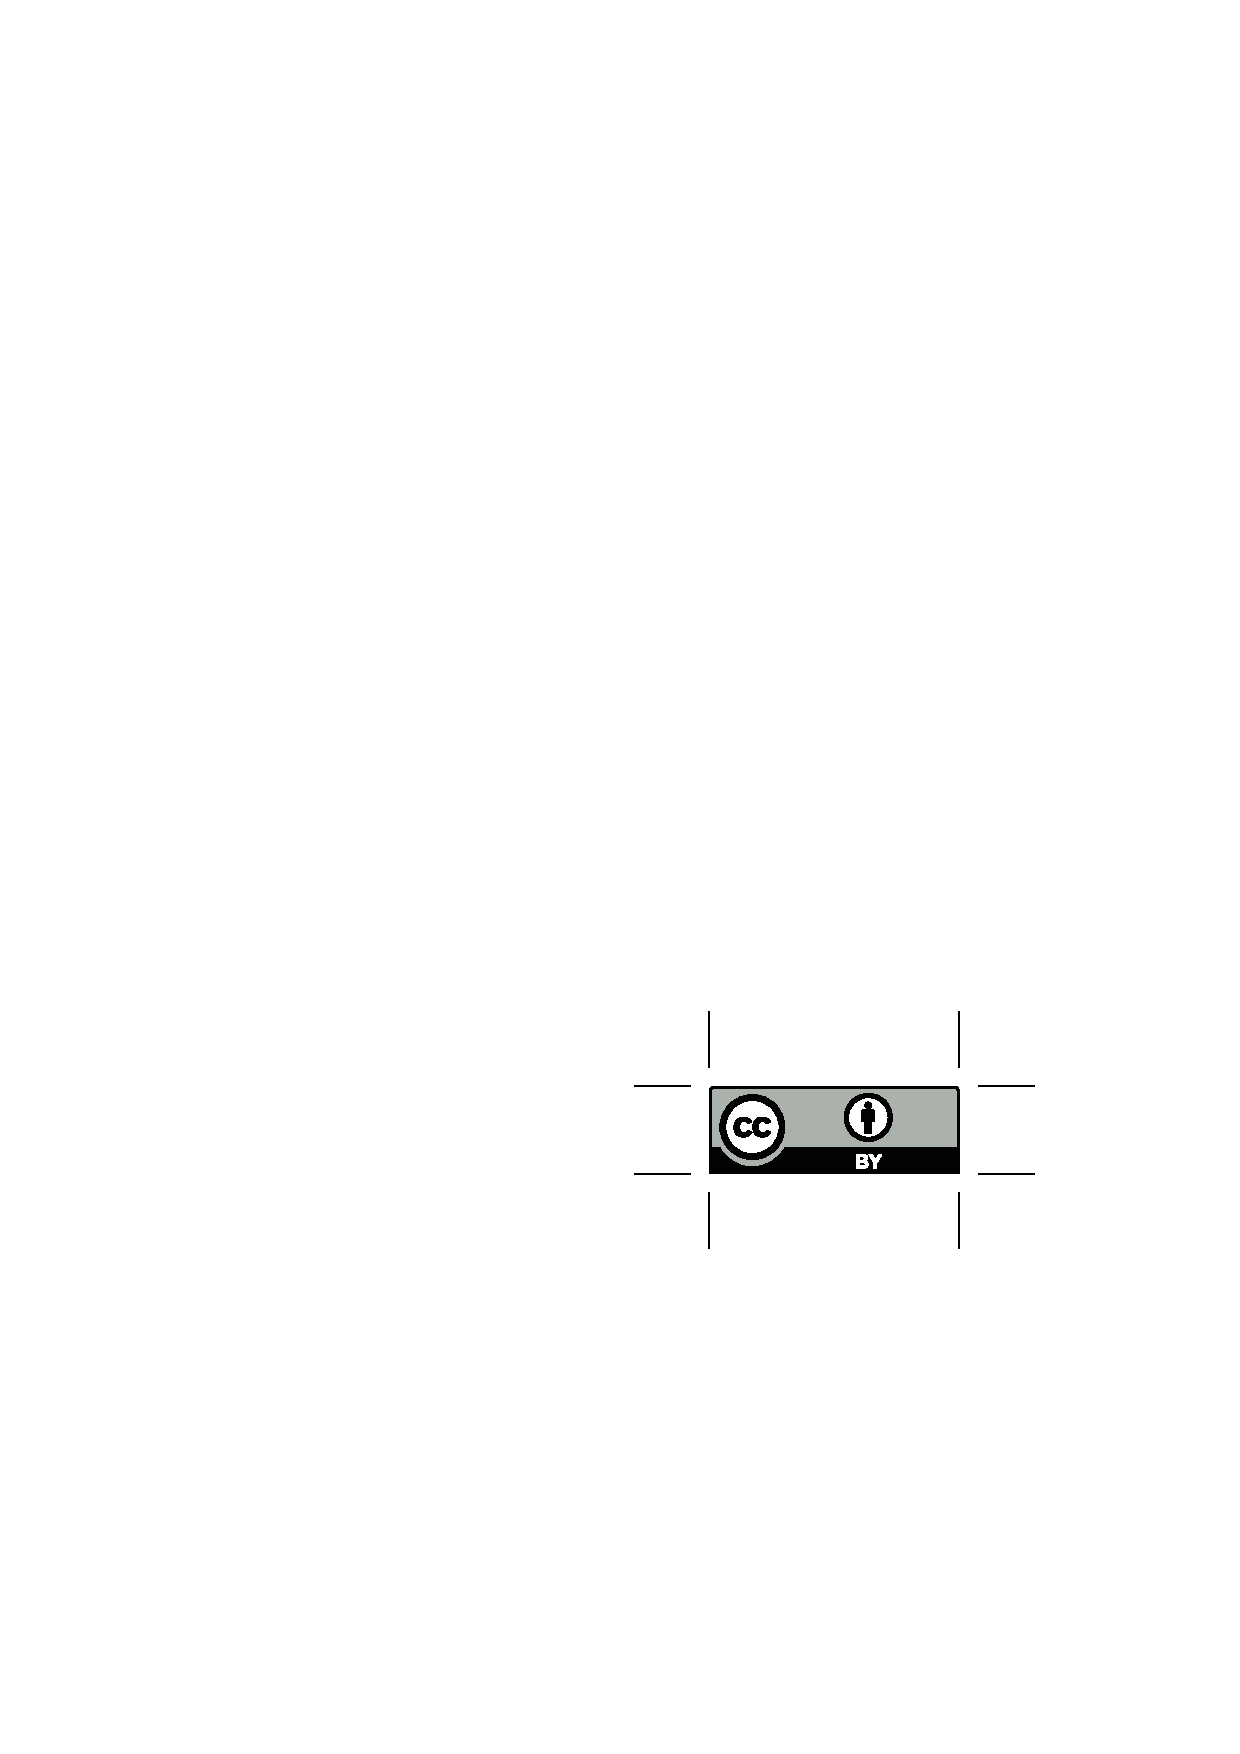
\includegraphics[width=0.90\textwidth]{by}}
  \end{minipage}\hfill
  \begin{minipage}{0.8\columnwidth}
   \href{https://creativecommons.org/licenses/by/4.0/}{This work is licensed under a Creative Commons Attribution International 4.0 License.}
  \end{minipage}
  \vspace{5pt}
}
\makeatother

\setcopyright{ifaamas}
\acmConference[AAMAS 2027]{Proc.\@ of the 26th International Conference
on Autonomous Agents and Multiagent Systems (AAMAS 2027)}{3--7 May 2027}{Hanoi, Vietnam}{M.~Baldoni, F.~Fang, W.~Yeoh, N.~Yorke-Smith (eds.)}
\copyrightyear{2027}
\acmYear{2027}
\acmDOI{}
%\acmPrice{}
\acmISBN{}

%%%%%%%%%%%%%%%%%%%%%%%%%%%%%%%%%%%%%%%%%%%%%%%%%%%%%%%%%%%%%%%%%%%%%%%%

%%% == IMPORTANT ==
%%% Use this command to specify your OpenReview submission number.
%%% In anonymous mode, it will be printed on the first page.

\acmSubmissionID{<<OpenReview submission id>>}

\submissionType{Research Paper Track}

\title[When Does MARL Help Context Curation?]{When Does Multi-Agent Reinforcement Learning Help Context Curation? Cost-Aware Retriever Agents for Frozen LLM Readers}

%%% Authors are hidden in anonymous mode; fill in for the camera-ready version.
\author{Anonymous Author(s)}
\affiliation{
  \institution{Anonymous Institution}
  \city{Anonymous City}
  \country{Anonymous Country}}
\email{anonymous@example.org}

\begin{abstract}
Retrieval-augmented generation (RAG) usually hands a frozen large language model (LLM) a fixed number of retrieved text chunks, although every chunk costs tokens and irrelevant ones invite wrong answers. We ask when multi-agent reinforcement learning (MARL) is worth using to decide which chunks to send. In \method{}, five retrievers (lexical, static word vectors, two dense encoders and a cross-encoder) act as agents that take turns writing chunks to a shared context under a token price, trained with a team reward paid as each chunk's marginal contribution. In a validation specified before the experiments (CRAG, HotpotQA, MuSiQue; 411 cross-validated RL runs; tests over dataset--seed clusters with Holm correction), the multi-agent team beat a centralized RL agent in all 15 clusters and learned to silence a misleading retriever (AUC 0.42; at most 2\% of the messages) and a random one (at most 0.1\%). Cooperative credit mattered only where evidence was redundant: on CRAG, selfish rewards made agents send 3--7$\times$ more tokens and turned the team reward negative ($-0.28$ vs.\ $0.33$), as our analysis predicts. With the same inputs the team beat a supervised selector in 15 of 15 clusters; with richer hand-made features the two tied. Training with simulated agent failures cut the loss from losing the strongest retriever by 61--95\%. On CRAG the team is statistically tied with the best retrieval pipelines (e.g.\ ColBERTv2, Search-R1) in answer score and RAGAS while sending 240--480 instead of 1{,}100--1{,}530 input tokens per question; training takes 16 minutes and about 4\,Wh on one CPU core. A perfect selector would add only 0.01--0.03 to the mean RAGAS score: with a frozen reader and one to three chunks, the reader, not the selector, sets the ceiling.
\end{abstract}

\keywords{Retrieval-augmented generation, Multi-agent reinforcement learning, Credit assignment, Cost-aware communication, Metareasoning, RAGAS, Sustainability}

%%% Author-defined commands
\newcommand{\method}{MA-Chunk}
\theoremstyle{plain}
\newtheorem{proposition}{Proposition}
\theoremstyle{definition}
\newtheorem{definition}{Definition}

\begin{document}

\maketitle


% ---------------------------------------------------------------------------
\section{Introduction}

Retrieval-Augmented Generation (RAG)~\cite{lewis2020rag} lets a frozen large language model (LLM), the \emph{reader}, answer from retrieved text segments (\emph{chunks}). Most pipelines pass the top-$k$ chunks of one retriever, with the same $k$ for every question. This wastes a scarce resource. Tokens are not free: on CRAG, the retrieval baselines we compare against send the reader 1{,}100--1{,}750 input tokens per question. And more context is not always better: long contexts are used unevenly~\cite{liu2024lost}, and irrelevant chunks invite confident wrong answers.

Choosing what to send is naturally a multi-agent problem. A lexical retriever (BM25), a static word-vector retriever, dense bi-encoders and a cross-encoder each rank the same candidates differently, and they are not equally reliable: on CRAG, the area under the ROC curve (AUC) of their scores for a useful chunk ranges from 0.42, worse than chance, to 0.82. Deciding which retriever should speak, how much, and when to stay silent is a problem of cost-aware communication~\cite{lin2026cobe}, of metareasoning about when information is worth its cost~\cite{budd2026thinkfast,russell1991metareasoning}, of redundancy among agents~\cite{zhang2026d3mas} and of credit assignment~\cite{nagpal2025llmmca,foerster2018coma}. MARL fits this description, but whether it beats simpler alternatives has to be measured, not assumed.

Our starting point is a negative result. A previous single-agent RL chunk selector read chunks in page order, inspected only 15--80 of the $\approx$1{,}450 chunks of a CRAG question, and relied on a signal that ranks useful chunks below chance (Section~\ref{sec:diagnosis}). We reformulate the task as cooperation among retriever agents and test it with a protocol written before the experiments: ten hypotheses on the reward, credit, turn order, messages, robustness, transfer, sensitivity and, crucially, whether RL is needed at all. Our contributions and main findings:
\begin{enumerate}
  \item \textbf{Formulation.} A Dec-POMDP in which retrievers are agents writing to a shared context, with a team reward paid as marginal contributions (Proposition~\ref{prop:telescope}) and a condition under which selfish and cooperative rewards coincide (Proposition~\ref{prop:modular}).
  \item \textbf{Environment.} A Gymnasium-compatible multi-agent environment for context curation, released with candidate pools and usefulness labels for CRAG (250 questions), HotpotQA and MuSiQue (1{,}000 each). Training needs no LLM call, and the experimental factors are switches: reward (marginal, terminal, selfish, precision-aware), turn order (round-robin, random, confidence), messages and message noise, agent failure and dropout, rich observations and a random distractor agent. 27 property tests check budgets, termination and that rewards sum to the team objective.
  \item \textbf{When MARL helps.} The multi-agent team beats a centralized RL agent in 15/15 dataset--seed clusters; selfish credit causes 3--7$\times$ more tokens exactly where Proposition~\ref{prop:modular} predicts (CRAG) and changes nothing where it predicts no effect; training with agent failures cuts the worst failure loss by 61--95\%.
  \item \textbf{Why RL, and how much curation can do.} RL beats a supervised selector with the same inputs (15/15 clusters) but ties with richer engineered features. Even oracle contexts leave 29--39\% wrong answers, so learning when \emph{not} to answer is the largest lever (CRAG score $0.068\to0.142$).
  \item \textbf{A fair RAGAS comparison and its ceiling.} Evaluating all methods at the same context granularity removes an artifact that inflated two baselines' context precision (0.29 and 0.38 become 0.54 and 0.52 when scored as one block). A precision-aware reward raises context precision, and a perfect selector would add only 0.01--0.03 to the mean RAGAS score.
  \item \textbf{Cost.} Training takes 16 minutes and $\approx$4\,Wh on one CPU core and a decision 5--8\,ms (CodeCarbon); scoring the candidates ($\approx$6\,s per CRAG question on a GPU) dominates the cost.
\end{enumerate}

% ---------------------------------------------------------------------------
\section{Related Work}

\paragraph{Agentic and multi-agent RAG.}
Search-R1~\cite{jin2025searchr1} trains an LLM with RL to interleave reasoning and search; DeepRetrieval~\cite{jiang2025deepretrieval} learns query reformulation with RL; s3~\cite{jiang2025s3} trains a searcher for a frozen generator. In the AAMAS community, Mujica-MyGo~\cite{wu2026mujica} decomposes multi-turn RAG into cooperative sub-interactions and post-trains the LLM, and SCMRAG~\cite{agrawal2025scmrag} adds self-corrective agents over a dynamic knowledge graph. These approaches train or prompt the LLM; \method{} keeps the reader frozen (it can be an API model) and learns lightweight curation agents that train on a CPU in minutes.

\paragraph{Cost-aware communication and metareasoning.}
COBE~\cite{lin2026cobe} treats communication as a dual objective (reward vs.\ usage) and operates on the empirical Pareto front; we adopt this view (a message is a chunk, its cost its tokens) and compare methods on utility--cost frontiers. Online metareasoning~\cite{budd2026thinkfast,russell1991metareasoning} and cost-aware escalation~\cite{bachar2026lpp} learn when computation or a costly resource is worth it, as our \textsc{stop} action and abstention agent do. Token efficiency is increasingly a first-class metric in LLM multi-agent systems~\cite{liu2026groupdebate,benkhaled2026g2cp,xiao2026routerhgc}, and D$^3$MAS~\cite{zhang2026d3mas} documents knowledge redundancy among agents.

\paragraph{Credit assignment.}
Counterfactual and difference rewards~\cite{wolpert2001difference,foerster2018coma} credit each agent with its contribution to the team outcome; LLM critics have also been used~\cite{nagpal2025llmmca}. We compare marginal credit with exact Shapley values and with selfish rewards.

% ---------------------------------------------------------------------------
\section{Problem Formulation}

\paragraph{Intuition.} Think of the reader's context window as a shared channel. Each retriever agent holds its own ranked list of eight candidate chunks. Agents take turns: the agent on turn looks at its current candidate and \emph{sends} it to the channel, \emph{skips} it, or \emph{stops} for good. Every chunk sent costs $\lambda$ per 1{,}000 tokens, and the team gains utility when the channel holds the evidence the question needs. Usefulness labels are computed once, so training never calls the reader.

\paragraph{Formalization.} A question $q$ has a pool of candidate chunks $\mathcal{C}$ (on CRAG, $\approx$1{,}450 per question, of which each agent considers its own top 8). The reader answers $q$ from a context $S\subseteq\mathcal{C}$; chunk $c$ costs $\tau(c)$ tokens. Let $G\subseteq\mathcal{C}$ be the useful evidence (Section~\ref{sec:setup}); the utility of a context is the covered fraction
\begin{equation}
U(S)=\min\!\left(1,\ \frac{|S\cap G|}{n_G}\right),
\end{equation}
where $n_G$ is the number of evidence pieces required ($n_G=1$ on CRAG; the number of gold supporting paragraphs on multi-hop QA).

\begin{definition}[Curation Dec-POMDP]
A tuple
\[\langle \mathcal{I}, \mathcal{X}, b_0, \{\mathcal{A}_i\}, P, R, \{\Omega_i\}, O, \gamma=1\rangle,\]
where
the agents $\mathcal{I}=\{1,\dots,n\}$ are retrievers, agent $i$ holding its top-$M$ list $L_i$ ranked by its score $f_i(q,\cdot)$;
a state $x\in\mathcal{X}$ holds the query $q\sim b_0$, the channel $S$, each agent's position in its list and whether it is still active;
the actions are $\mathcal{A}_i=\{\textsc{skip},\textsc{send},\textsc{stop}\}$;
$P$ is turn-based: the acting agent sends its current candidate to $S$, moves to its next candidate, or leaves, and candidates already in $S$ are skipped;
$R$ is the team reward below;
and the local observation $o_i\in\Omega_i$ contains the agent's identity, its own score and rank, cross-agent agreement, the redundancy $\max_{c'\in S}\cos(e(c),e(c'))$, channel occupancy, message counts, list progress and $\tau(c)$; with \emph{messages}, also the other agents' scores for the candidate under discussion.
An episode ends when every agent has stopped or exhausted its list, or $S$ reaches 10 chunks or 2{,}000 tokens (so the horizon is finite).
\end{definition}

\noindent We use $n=5$ retrievers: BM25 (sparse), spaCy \texttt{en\_core\_web\_md} cosine (static word vectors, the prior selector's signal), MiniLM and E5 (dense bi-encoders) and a cross-encoder reranker. No observation contains a label or the gold answer.

\paragraph{Team reward and credit.}
The team objective is $R(S)=U(S)-\lambda\,\tau(S)/1000$, with $\tau(S)=\sum_{c\in S}\tau(c)$ and a token price $\lambda\ge0$. It is paid at each \textsc{send} of $c$ as the marginal contribution
\begin{equation}
r_t=U(S_t\cup\{c\})-U(S_t)-\lambda\,\tau(c)/1000,
\end{equation}
and $r_t=0$ for \textsc{skip} and \textsc{stop}.

\begin{proposition}\label{prop:telescope}
In every episode $\sum_t r_t=R(S_T)$, and the reward credited to agent $i$ equals the marginal utility of its own messages minus their cost.
\end{proposition}
\begin{proof}
The utility increments telescope to $U(S_T)-U(\emptyset)=U(S_T)$, the costs add up to $\lambda\tau(S_T)/1000$, and each term is produced by exactly one \textsc{send}.
\end{proof}

\noindent The \emph{selfish} alternative pays each sender for its own chunk regardless of the team, $r^{\mathrm{ind}}_t=\mathbf{1}[c\in G]/n_G-\lambda\tau(c)/1000$.

\begin{proposition}\label{prop:modular}
If $U$ is modular on the reachable contexts, i.e.\ $U(S\cup\{c\})-U(S)=\mathbf{1}[c\in G]/n_G$ for every reachable $S$ and $c\notin S$, then $r^{\mathrm{ind}}_t=r_t$ at every step and both rewards define the same learning problem. If $U$ saturates ($|G|>n_G$, e.g.\ several chunks each containing the answer), $r^{\mathrm{ind}}$ pays every redundant useful message that $r_t$ prices at $-\lambda\tau(c)/1000$.
\end{proposition}
\begin{proof}
Immediate from the definitions: the two rewards differ only by $\mathbf{1}[c\in G]/n_G-(U(S\cup\{c\})-U(S))$, which is zero under modularity and equal to $1/n_G$ for a useful $c$ sent after saturation.
\end{proof}

\noindent On multi-hop QA, $G$ holds exactly the $n_G$ distinct gold paragraphs, so $U$ never saturates and is modular; on CRAG several chunks can each contain the answer ($|G|>1=n_G$), so $U$ saturates at the first useful chunk. Proposition~\ref{prop:modular} thus predicts that credit design matters on CRAG only.

\paragraph{Metareasoning gate.}
Under the CRAG rule~\cite{yang2024crag} a correct answer scores $+1$, a wrong one $-1$ and an abstention $0$; the \emph{CRAG score} of a method is \%correct $-$ \%incorrect. A gate agent observes query-level evidence before the reader is called and chooses \textsc{answer} or \textsc{abstain}, with the CRAG score of the outcome as reward. We compare a PPO gate (13 evidence features) with a one-parameter threshold policy on the best cross-encoder score, both trained on training folds only.

% ---------------------------------------------------------------------------
\section{Method}

All curation agents share one policy network (agent identity in the observation), trained with PPO~\cite{schulman2017ppo} on the turn-based episodes: two 64-unit layers, learning rate $3\cdot10^{-4}$, entropy coefficient $0.01$, $\gamma=1$, $2\cdot10^{5}$ steps per fold. Parameter sharing with identity features is the standard cooperative MARL baseline~\cite{yu2022mappo}; we also train the same team with A2C, DQN and Recurrent PPO. Hyperparameters were fixed before the experiments and are identical for every variant.

Usefulness is labelled once per candidate: on CRAG by an LLM judge that sees the gold answer (7{,}492 chunks; 79.6\% of the questions have at least one useful chunk in the pool), on multi-hop QA by the gold supporting paragraphs. Training therefore needs no API call. We compare five variants: \textbf{MA} (each agent sees only its own score), \textbf{MA+msg} (agents also receive the other agents' scores as messages; our default), \textbf{MA+msg-rich} (messages also carry per-question z-scores and log-ranks), \textbf{failure-aware} (during training each agent fails with probability $0.2$ per episode, and observations say which agents are present), and the ablation \textbf{Single}, one centralized agent that walks the fused (reciprocal-rank-fusion, RRF) list of all five retrievers and sees all five scores.

\paragraph{Precision-aware variant (MA-Chunk-P).}
RAGAS context precision~\cite{es2024ragas} is the average precision of the context list, $\mathrm{AP}(S)=\sum_k P@k\,v_k/\sum_k v_k$ with $v_k$ the usefulness of the $k$-th chunk, so it rewards evidence that comes first. We add it to the team objective, $R_P(S)=U(S)+\beta\,\mathrm{AP}(S)-\lambda\tau(S)/1000$ with $\beta=1$, still paid as marginal contributions (the argument of Proposition~\ref{prop:telescope} holds for any function of the ordered channel; $\mathrm{AP}$ is computed with the utility labels exactly as RAGAS computes it, which we verified numerically), and let the agent with the most confident current candidate speak first.

% ---------------------------------------------------------------------------
\section{Experimental Setup}\label{sec:setup}

\paragraph{Data.}
CRAG~\cite{yang2024crag}: 250 questions (five domains) with full search-result pages, chunked into segments of at most 500 characters. HotpotQA~\cite{yang2018hotpotqa} and MuSiQue~\cite{trivedi2022musique}: 1{,}000 development questions each (FlashRAG release). HotpotQA candidates are the 10 provided paragraphs (retrieved in this release; both gold paragraphs are present for about 30\% of the questions); MuSiQue candidates are each question's top-20 paragraphs by BM25 over a closed corpus of all 16{,}301 support paragraphs, without injecting the gold ones. The maximum reachable utility is $0.56$ and $0.58$, respectively.

\paragraph{Protocol and statistics.}
Every learned component is evaluated with 5-fold cross-validation (stratified by domain on CRAG); the seed fixes the folds, so variants trained with the same seed see identical splits. Ten hypotheses and their decision criteria were written down before the validation; deviations are reported. Runs that share a dataset and a seed are not independent, so our statistical unit is the \emph{cluster} (dataset, seed): for each cluster we average the paired difference in team reward over the two token prices $\lambda\in\{0.3,1\}$, and compare clusters with an exact Wilcoxon signed-rank test (9 clusters for ablations, 15 for the main comparisons), with 95\% cluster-bootstrap intervals and Holm correction within each family of related tests. End-task comparisons are paired per question (Wilcoxon, scores averaged over seeds). Re-running 36 configurations with the final code reproduced the original results bit for bit, and the training return changes by less than 0.3\% (median) over the last 10\% of training.

\paragraph{Reader, judge and their reliability.}
All methods, including baselines, are re-read by the same frozen reader (\texttt{gpt-5-nano}, minimal reasoning, one prompt) and judged by the same model in CRAG style (\emph{correct}, \emph{incorrect}, \emph{missing}; refusals are detected deterministically). Re-judging 300 random answers with a second model (\texttt{gpt-4.1-nano}) gave 97.3\% agreement (Cohen's $\kappa=0.96$), so end-task conclusions do not hinge on the judge. Re-labelling 300 CRAG chunks gave $\kappa=0.64$: the second model is stricter (it confirms 65\% of the positives and flips 1.3\% of the negatives), a source of label noise on CRAG that does not affect the gold-labelled multi-hop sets.

\paragraph{Baselines.}
On CRAG, BM25, FAISS, ColBERTv2~\cite{santhanam2022colbertv2}, DeepRetrieval~\cite{jiang2025deepretrieval} (FAISS/BM25), Search-R1~\cite{jin2025searchr1} and the four prior single-agent RL policies, each with its own chunks. On every dataset and on the same pool as \method{}: top-$k$ of each retriever, RRF top-$k$, an oracle that sends the best-ranked useful chunk, and \emph{supervised selectors} (logistic regression or gradient boosting predicting usefulness, followed by a decision-theoretic greedy rule that sends chunks while the expected marginal utility exceeds $\lambda\tau(c)/1000$, i.e.\ the same objective), using either the agents' features (\emph{parity}) or richer engineered features (per-query z-scores and log-ranks).

\paragraph{RAGAS.}
We also report the five RAGAS metrics (ragas 0.2.15, judge \texttt{gpt-5-nano}) and their per-question mean (RAGAS-5) for every method, with the common reader. Context lists are compared at the same granularity ($\le$500 characters per context); faithfulness is undefined for empty answers (3--16\% of the questions, depending on the method) and excluded from the mean. CRAG uses all 250 questions, HotpotQA and MuSiQue a fixed random sample of 300 each. Comparisons with MA+msg use \emph{budget-matched} token prices, chosen from chunk counts alone before any LLM evaluation; hypotheses, decision criteria and amendments were written down before the corresponding results.

\paragraph{Sustainability.}
Energy and emissions are measured with CodeCarbon in process mode on a shared server (Intel Xeon Gold 6326, NVIDIA L40S; local grid, 98\,g CO$_2$/kWh). RAPL counters are not readable without root, so CPU power is estimated from the processor's thermal design power and the process's CPU share; CPU-only jobs report CPU and RAM energy, and GPU jobs report the energy of the device they use, an upper bound because the device was shared.

% ---------------------------------------------------------------------------
\section{Results}

\subsection{Why the single-agent selector failed}\label{sec:diagnosis}

\emph{Short answer: it read chunks in page order and trusted a signal that is worse than chance.} The prior single-agent policies walked a page in document order and stopped when the budget filled: they inspected 15--80 of $\approx$1{,}450 chunks, recurrent PPO took the first chunks of the page in 90\% of the episodes, and PPO and recurrent PPO always selected exactly 10. Only 4--7\% of their selections were among the page's top 10 by their own reward signal. Ranking the whole page by that signal did not help either (CRAG score of its top-5: $0.040$; of the policies: $-0.040$ to $0.068$), because the signal itself is poor: its static word-vector component has an AUC of $0.42$ for usefulness on the labelled CRAG pool (Table~\ref{tab:signals}).

\begin{table}[t]
\centering\small
\caption{AUC of each agent's score for a useful chunk, and share of \textsc{send} messages of the trained team (MA+msg, $\lambda=1$, random turn order to remove first-mover bias; mean of 3 seeds).}
\label{tab:signals}
\setlength{\tabcolsep}{3.5pt}
\begin{tabular}{ll ccccc}
\toprule
 & & BM25 & spaCy & MiniLM & E5 & Cross-enc. \\
\midrule
\multirow{2}{*}{CRAG} & AUC & 0.54 & \textbf{0.42} & 0.72 & 0.76 & 0.82 \\
 & Messages & 1.1\% & 0.8\% & 2.7\% & 30.1\% & 65.4\% \\
\midrule
\multirow{2}{*}{HotpotQA} & AUC & 0.84 & \textbf{0.56} & 0.87 & 0.95 & 0.93 \\
 & Messages & 18.6\% & 1.4\% & 13.0\% & 37.5\% & 29.4\% \\
\midrule
\multirow{2}{*}{MuSiQue} & AUC & 0.79 & \textbf{0.51} & 0.92 & 0.91 & 0.93 \\
 & Messages & 16.2\% & 2.0\% & 19.0\% & 26.5\% & 36.2\% \\
\bottomrule
\end{tabular}
\end{table}

\subsection{Learning and the utility--token frontier}

Training converges quickly: across datasets and variants the return plateaus within 50--100k steps per fold and stays flat afterwards (Figure~\ref{fig:training}). Figure~\ref{fig:frontier} plots the evidence each method puts in the context against the tokens it spends; higher and further left is better. On both multi-hop datasets the team lies above every static top-$k$ selector: averaged over the token window that all methods cover, its utility is 0.459 vs.\ 0.381 for cross-encoder top-$k$ on HotpotQA and 0.457 vs.\ 0.399 on MuSiQue, and also above the centralized agent (0.443 and 0.444). On CRAG the team and cross-encoder top-$k$ are level (0.542 vs.\ 0.548): the team is ahead at 100--200 tokens, the cross-encoder at about 600. The supervised selector with rich features is the strongest competitor on multi-hop QA (0.486 and 0.470; Appendix~\ref{app:frontier}).

\begin{figure*}[t]
\centering
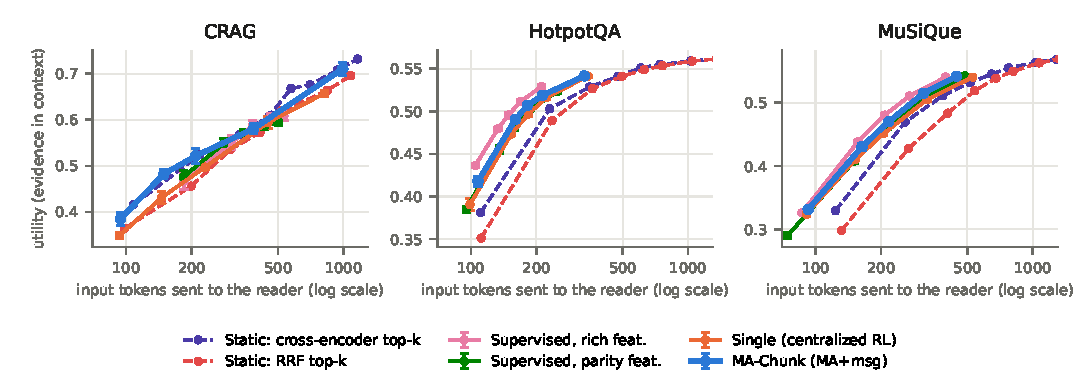
\includegraphics[width=0.92\linewidth]{figs/frontier.pdf}
\caption{Utility (fraction of the needed evidence in the context) vs.\ input tokens sent to the reader, on the test folds. Learned methods: one point per token price $\lambda\in\{2,1,0.6,0.3,0.1\}$ (mean $\pm$ sd over seeds); static selectors: one point per $k$.}
\label{fig:frontier}
\Description{Three panels (CRAG, HotpotQA, MuSiQue) plotting the fraction of needed evidence in the context against input tokens on a log scale, for static top-k selectors, the supervised selectors, the centralized RL agent and MA-Chunk.}
\end{figure*}

\begin{figure*}[t]
\centering
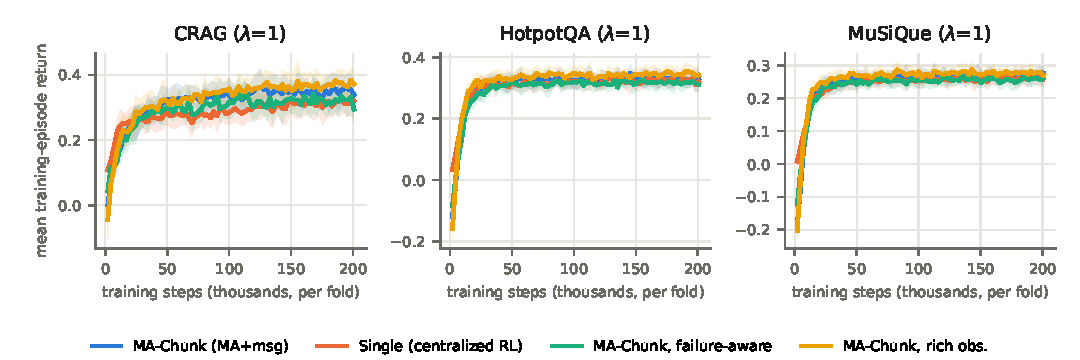
\includegraphics[width=0.92\linewidth]{figs/training_curves.pdf}
\caption{Training curves at $\lambda=1$: mean training-episode return (mean $\pm$ sd over seeds and folds) of the variants trained with PPO (the failure-aware curve includes episodes with failed agents). Curves of the four RL algorithms are in Appendix~\ref{app:algos}.}
\label{fig:training}
\Description{Three panels of mean training-episode return versus training steps for MA-Chunk variants trained with PPO; all curves rise quickly and plateau within 50 to 100 thousand steps.}
\end{figure*}

\subsection{Does the multi-agent decomposition help?}

\emph{Short answer: yes, in every cluster.} MA+msg beat the centralized Single agent in all 15 clusters (Table~\ref{tab:validation}: $+0.015$ team reward, about 4\% of the Single agent's mean and up to 14\% on CRAG at $\lambda=1$; $p_{\mathrm{Holm}}<0.001$), and the gap persisted when both received rich observations (9 of 9 clusters). Explicit score messages added only a small, non-significant gain ($+0.003$, 7 of 9 clusters). The team also learned whom to listen to (Table~\ref{tab:signals}). With an order-neutral (random) turn order, the share of messages follows signal quality: on CRAG the cross-encoder (AUC 0.82) sends 65\% of the messages and the misleading spaCy agent (AUC 0.42) under 1\%; across datasets spaCy never exceeds 2.0\%, and a sixth agent with random scores sent at most 0.1\% of the messages while leaving the team reward unchanged. We report shares under random order because round-robin turns favour whoever speaks first when the agents' lists overlap (on HotpotQA, BM25, first in the cycle, sends 45\%).

% AUTO-GENERATED by scripts/paper/tables_validation.py
\begin{table}[t]
\centering\footnotesize
\caption{Pre-specified comparisons at the cluster level (dataset $\times$ seed; team reward averaged over $\lambda\in\{0.3,1\}$). $\Delta$: mean paired difference $A-B$ in units of $10^{-3}$ team reward, with 95\% cluster-bootstrap CI; W/L: clusters won/lost by $A$; exact Wilcoxon signed-rank $p$, Holm-corrected within each family.}
\label{tab:validation}
\setlength{\tabcolsep}{2.5pt}
\begin{tabular}{l r c r}
\toprule
$A$ vs.\ $B$ & $\Delta$ [95\% CI] & W/L & $p_{\mathrm{Holm}}$ \\
\midrule
\multicolumn{4}{l}{\emph{Decomposition}} \\
\quad MA+msg vs.\ Single & 15.3 [11.1, 20.0] & 15/0 & $<$0.001 \\
\quad MA+msg-rich vs.\ Single-rich & 6.1 [3.3, 9.9] & 9/0 & 0.008 \\
\quad MA+msg vs.\ MA (no messages) & 3.3 [$-$0.1, 6.3] & 7/2 & 0.098 \\
\addlinespace[2pt]
\multicolumn{4}{l}{\emph{Reward and credit}} \\
\quad marginal vs.\ terminal reward & 7.2 [4.1, 11.1] & 9/0 & 0.008 \\
\quad marginal vs.\ selfish reward & 337.6 [332.4, 341.5]$^{\dagger}$ & 3/0 & 0.250 \\
\addlinespace[2pt]
\multicolumn{4}{l}{\emph{Orchestration}} \\
\quad round-robin vs.\ random order & $-$0.1 [$-$3.6, 3.7] & 3/6 & 0.496 \\
\quad round-robin vs.\ confidence order & $-$4.1 [$-$7.2, $-$1.7] & 0/9 & 0.008 \\
\addlinespace[2pt]
\multicolumn{4}{l}{\emph{Robustness and sensitivity}} \\
\quad 5 agents vs.\ +random agent & $-$0.8 [$-$3.3, 1.0] & 6/3 & 1.000 \\
\quad top-8 vs.\ top-4 lists & 0.1 [$-$4.6, 6.9] & 2/7 & 1.000 \\
\quad top-8 vs.\ top-12 lists & 3.9 [0.6, 9.5] & 8/1 & 0.078 \\
\quad standard vs.\ failure-aware (clean) & 1.7 [$-$0.6, 4.5] & 5/4 & 1.000 \\
\addlinespace[2pt]
\multicolumn{4}{l}{\emph{Why RL?}} \\
\quad MA+msg vs.\ supervised (parity) & 18.7 [11.9, 26.1] & 15/0 & $<$0.001 \\
\quad MA+msg vs.\ supervised GBM (rich) & 7.5 [$-$4.6, 21.8] & 5/10 & 1.000 \\
\quad MA+msg vs.\ supervised logistic (rich) & $-$2.1 [$-$10.1, 6.1] & 5/10 & 1.000 \\
\quad MA+msg-rich vs.\ supervised GBM (rich) & 11.9 [$-$0.7, 26.3] & 5/4 & 1.000 \\
\quad MA+msg-rich vs.\ supervised logistic (rich) & 1.5 [$-$3.8, 7.8] & 3/6 & 1.000 \\
\bottomrule
\multicolumn{4}{p{0.97\columnwidth}}{\scriptsize $^{\dagger}$CRAG only, where utility saturates (3 clusters; range over clusters instead of CI). On the 6 multi-hop clusters both rewards produced identical policies, as Proposition~\ref{prop:modular} predicts.}
\end{tabular}
\end{table}


\subsection{Reward, credit and the social dilemma}

\emph{Short answer: paying each chunk's marginal contribution works best, and selfish rewards fail exactly where theory says they should.} A single terminal team reward learned slightly but consistently worse than the marginal reward (all 9 clusters, $p_{\mathrm{Holm}}=0.008$). Selfish rewards behaved as Proposition~\ref{prop:modular} predicts (Table~\ref{tab:dilemma}). On multi-hop QA, where utility is additive, they produced the same policies as the cooperative reward. On CRAG, where one useful chunk suffices and further copies add nothing, they created a social dilemma in every seed: agents sent 3.0$\times$ ($\lambda=0.3$) and 6.7$\times$ ($\lambda=1$) more tokens, and at $\lambda=1$ the team reward fell from $0.330$ to $-0.284$. With three CRAG seeds a cluster test cannot reach significance (exact $p=0.25$ is the smallest attainable value), but the gap was $+0.33$ to $+0.34$ in every seed. Marginal credit sums exactly to the team utility but depends on who speaks first: on CRAG its rank correlation with exact Shapley values is $0.77$ ($\lambda=0.3$) and $0.90$ ($\lambda=1$), and on the additive multi-hop utilities it equals the Shapley value. Selfish credit ranks the agents correctly ($\rho=0.98$) but over-pays them (error 0.18--0.19 vs.\ 0.03--0.07), which is what drives over-sending.

\begin{table}[t]
\centering\small
\caption{Cooperative (marginal) vs.\ selfish rewards on CRAG, where utility saturates (mean of 3 seeds). Credit: Spearman correlation / mean absolute error between each team's credit scheme and exact Shapley values.}
\label{tab:dilemma}
\setlength{\tabcolsep}{3pt}
\begin{tabular}{l cc cc}
\toprule
 & \multicolumn{2}{c}{$\lambda=0.3$} & \multicolumn{2}{c}{$\lambda=1.0$} \\
\cmidrule(lr){2-3}\cmidrule(lr){4-5}
 & Coop. & Selfish & Coop. & Selfish \\
\midrule
Team reward & \textbf{0.462} & 0.401 & \textbf{0.330} & $-$0.284 \\
Tokens sent & 375 & 1{,}113 & 149 & 997 \\
Credit vs.\ Shapley ($\rho$ / MAE) & 0.77 / 0.07 & 0.98 / 0.19 & 0.90 / 0.03 & 0.98 / 0.18 \\
\bottomrule
\end{tabular}
\end{table}

\subsection{Orchestration, robustness and generalization}

\emph{Short answer: turn order and message noise matter little; losing the strongest agent matters a lot unless the team is trained for it.} Random turns matched round-robin, and letting the most confident agent speak first was slightly better in all 9 clusters ($+0.004$, $p_{\mathrm{Holm}}=0.008$) and reached the first useful chunk earlier (CRAG: turn 3.0 vs.\ 3.8); we keep round-robin as the default because it was fixed in advance, so our main results are slightly conservative. The size of each agent's list (4, 8 or 12) had no significant effect. Table~\ref{tab:robust} reports perturbations applied to trained teams at test time. Gaussian noise on the messages (scores lie in $[0,1]$) cost at most $0.015$ team reward at $\sigma=0.2$ and at most $0.056$ at $\sigma=0.5$, where the messaging team fell below the no-message team on MuSiQue, against our stated expectation. The real weakness was the failure of the dominant agent: removing the cross-encoder at test time dropped the team reward from $0.462$ to $0.085$ on CRAG and from $0.455$ to $0.131$ on HotpotQA, because the other agents had learned to defer to it and read its silence as ``irrelevant''. Training with random agent dropout and a presence mask met both pre-specified criteria in all six conditions: the worst single-agent failure loss fell by 61--95\% (e.g.\ CRAG, $\lambda=0.3$: $0.377\to0.034$), with no detectable change in clean team reward (5 vs.\ 4 clusters, $p=0.43$) or end-task score. Teams trained on one dataset and applied to another kept 64--103\% (median 91\%) of their in-domain team reward.

\begin{table}[t]
\centering\small
\caption{Robustness (team reward loss vs.\ clean; mean of seeds). Failure: worst single-agent failure at test time, standard vs.\ failure-aware training. Noise: Gaussian noise on messages.}
\label{tab:robust}
\setlength{\tabcolsep}{3pt}
\begin{tabular}{l c cc cc}
\toprule
 & & \multicolumn{2}{c}{Worst failure loss} & \multicolumn{2}{c}{Noise loss} \\
\cmidrule(lr){3-4}\cmidrule(lr){5-6}
 & $\lambda$ & Standard & Failure-aware & $\sigma$=0.2 & $\sigma$=0.5 \\
\midrule
\multirow{2}{*}{CRAG} & 0.3 & 0.377 & \textbf{0.034} & 0.000 & 0.003 \\
 & 1.0 & 0.290 & \textbf{0.060} & 0.012 & 0.016 \\
\multirow{2}{*}{HotpotQA} & 0.3 & 0.324 & \textbf{0.017} & 0.002 & 0.007 \\
 & 1.0 & 0.326 & \textbf{0.026} & 0.004 & 0.025 \\
\multirow{2}{*}{MuSiQue} & 0.3 & 0.049 & \textbf{0.019} & 0.008 & 0.026 \\
 & 1.0 & 0.062 & \textbf{0.022} & 0.015 & 0.056 \\
\bottomrule
\end{tabular}
\end{table}

\subsection{Why reinforcement learning?}

\emph{Short answer: RL wins when both see the same information, and ties when the supervised model gets better features.} We gave a supervised selector the same labels, folds and objective: a classifier predicts each chunk's usefulness and a greedy rule sends chunks while the expected gain exceeds the token cost. With the agents' own inputs it lost to the team in all 15 clusters (by 0.019 team reward, $p_{\mathrm{Holm}}<0.001$): coordinated sequential decisions beat independent per-chunk decisions. With richer engineered features (per-question z-scores and log-ranks) the two were statistically tied (Table~\ref{tab:validation}): the supervised selector was ahead by 0.006--0.021 on the additive multi-hop utilities and behind by 0.05--0.09 on CRAG at $\lambda=1$. This matches expectations: for an additive objective with a linear cost, a greedy rule on well-calibrated probabilities is near-optimal, so coordination has room to help only when evidence interacts and budgets are tight. The choice of RL algorithm mattered less than the formulation (Appendix~\ref{app:algos}): PPO had the best mean rank (1.67 of 4; Friedman $p=0.013$) and the lowest variance across seeds, beat A2C in 9 of 9 clusters ($p_{\mathrm{Holm}}=0.012$) and tied with DQN and Recurrent PPO (6 of 9 clusters each, $p_{\mathrm{Holm}}=0.33$), which cost up to three times more to train.


% AUTO-GENERATED by scripts/paper/tables_ragas.py
\begin{table*}[t]
\centering\small
\caption{RAGAS on CRAG with a common reader and judge (\texttt{gpt-5-nano}); every context list at the same granularity ($\le$500 characters). Learned methods: 3 seeds averaged per question. RAGAS-5: mean of the five metrics (95\% bootstrap CI). $\Delta$: paired difference to MA-Chunk-P ($\lambda$=0.4) on common questions; $^{*}$: $p_{\mathrm{Holm}}<0.05$ (Wilcoxon, Holm over the rows). $^{\dagger}$Delivered as one $\approx$5{,}000-character block, re-split for evaluation; as a single block their context precision reads 0.54 (BM25) and 0.52 (Search-R1).}
\label{tab:ragas-crag}
\setlength{\tabcolsep}{3.5pt}
\begin{tabular}{ll r ccccc c r}
\toprule
Group & Method & Chunks & Faith. & Ans.\ rel. & Ans.\ corr. & Ctx.\ prec. & Ctx.\ rec. & RAGAS-5 [95\% CI] & $\Delta$ \\
\midrule
\multirow{6}{*}{Retrieval baselines} & BM25$^{\dagger}$ & 9.7 & 0.614 & 0.672 & 0.493 & 0.291 & 0.446 & 0.493 [0.452, 0.535] & $-$0.038 \\
 & FAISS & 10.0 & 0.432 & 0.585 & 0.440 & 0.175 & 0.294 & 0.373 [0.333, 0.413] & $-$0.140$^{*}$ \\
 & ColBERTv2 & 10.0 & 0.575 & 0.733 & 0.500 & 0.401 & 0.534 & 0.544 [0.505, 0.584] & 0.033 \\
 & DeepRetrieval+FAISS & 10.0 & 0.546 & 0.703 & 0.519 & 0.335 & 0.491 & 0.513 [0.474, 0.552] & 0.001 \\
 & DeepRetrieval+BM25 & 10.0 & 0.551 & 0.667 & 0.465 & 0.265 & 0.443 & 0.468 [0.429, 0.506] & $-$0.044$^{*}$ \\
 & Search-R1$^{\dagger}$ & 8.5 & 0.554 & 0.735 & 0.490 & 0.378 & 0.452 & 0.519 [0.486, 0.552] & 0.027 \\
\midrule
\multirow{4}{*}{Prior single-agent RL} & PPO & 10.0 & 0.498 & 0.663 & 0.470 & 0.243 & 0.359 & 0.440 [0.407, 0.473] & $-$0.052$^{*}$ \\
 & R-PPO & 10.0 & 0.494 & 0.660 & 0.472 & 0.231 & 0.423 & 0.447 [0.412, 0.482] & $-$0.045$^{*}$ \\
 & DDPG & 8.3 & 0.469 & 0.610 & 0.440 & 0.233 & 0.365 & 0.413 [0.376, 0.450] & $-$0.079$^{*}$ \\
 & SAC & 10.0 & 0.485 & 0.621 & 0.454 & 0.228 & 0.390 & 0.423 [0.388, 0.458] & $-$0.069$^{*}$ \\
\midrule
\multirow{3}{*}{Same pool} & Cross-enc.\ top-3 & 3.0 & 0.552 & 0.716 & 0.454 & 0.399 & 0.405 & 0.501 [0.466, 0.536] & 0.010 \\
 & RRF top-3 & 3.0 & 0.532 & 0.660 & 0.474 & 0.345 & 0.412 & 0.475 [0.437, 0.513] & $-$0.016 \\
 & Single, $\lambda$=0.6 & 2.4 & 0.520 & 0.649 & 0.449 & 0.341 & 0.391 & 0.460 [0.420, 0.500] & $-$0.032 \\
\midrule
\multirow{4}{*}{\method{}} & MA+msg, $\lambda$=0.3 & 3.5 & 0.527 & 0.700 & 0.454 & 0.360 & 0.429 & 0.492 [0.457, 0.524] & 0.000 \\
 & MA+msg, $\lambda$=1 & 1.5 & 0.481 & 0.657 & 0.423 & 0.343 & 0.364 & 0.446 [0.410, 0.482] & $-$0.046$^{*}$ \\
 & \textbf{MA-Chunk-P, $\lambda$=0.4} & 2.8 & 0.517 & 0.715 & 0.463 & 0.382 & 0.395 & 0.492 [0.457, 0.527] & ref. \\
 & MA-Chunk-P, $\lambda$=1.25 & 1.5 & 0.487 & 0.673 & 0.420 & 0.335 & 0.362 & 0.449 [0.414, 0.485] & $-$0.042$^{*}$ \\
\midrule
\multirow{1}{*}{Upper bound} & Oracle (useful chunk) & 1.0 & 0.478 & 0.676 & 0.494 & 0.456 & 0.457 & 0.502 [0.463, 0.541] & 0.010 \\
\bottomrule
\end{tabular}
\end{table*}


\begin{figure*}[t]
\centering
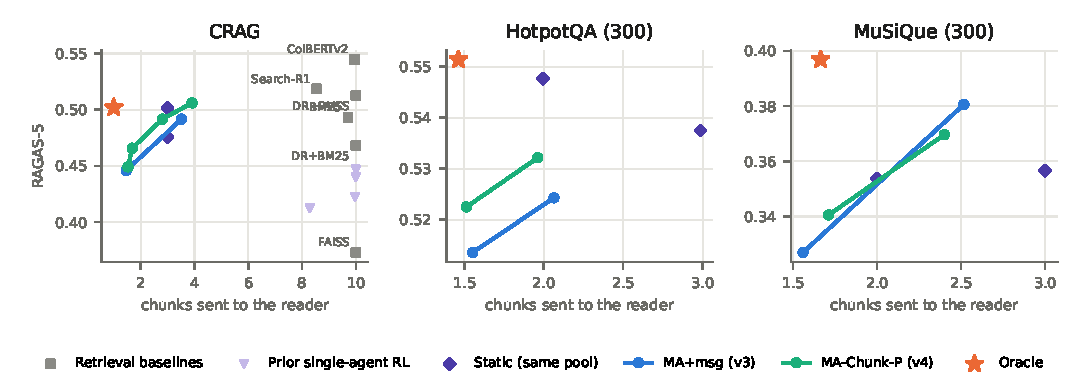
\includegraphics[width=0.92\linewidth]{figs/ragas_frontier.pdf}
\caption{RAGAS-5 vs.\ chunks sent to the reader (common reader and judge; learned methods: mean over 3 seeds per token price). MA+msg at $\lambda\in\{1,0.3\}$; MA-Chunk-P at budget-matched prices; static selectors on the same pool; retrieval baselines and prior single-agent RL policies (CRAG only); oracle sending the useful evidence. HotpotQA and MuSiQue: 300-question samples.}
\label{fig:ragas}
\Description{Three panels plotting the mean RAGAS score against the number of chunks sent to the reader for retrieval baselines, prior single-agent RL policies, static selectors, MA-Chunk, MA-Chunk-P and an oracle.}
\end{figure*}

\subsection{End task}

\emph{Short answer: good selectors tie, and the reader limits all of them.} Table~\ref{tab:endtask} reports the CRAG score (\%correct $-$ \%incorrect) and F1 with a common reader. On CRAG no method other than the oracle differs significantly from the team (paired tests against each of the ten external baselines: $p_{\mathrm{Holm}}\ge0.95$), and the team gets there with 240--480 input tokens, against 1{,}100--1{,}750 for the retrieval baselines and the prior RL policies (Appendix~\ref{app:crag}). On HotpotQA the learned selectors are ahead of the static ones: \method{} beat cross-encoder top-1 in all four configurations (paired Wilcoxon, $p\le0.008$) and RRF top-3 in three of four ($p\le0.05$), and tied with the supervised selectors (the logistic one had the highest mean, $0.184$ vs.\ $0.166$). On MuSiQue every method scores below zero, because the reader answers wrongly 39--50\% of the time. Even oracle contexts leave 29--39\% wrong answers across datasets, so the reader, not the context, limits the end task. The training signal is nonetheless well aligned with it: answers were correct 59--88\% of the time when the context contained the needed evidence and only 3--18\% when it did not.

\begin{table*}[t]
\centering\small
\caption{End task with a common reader and judge (\texttt{gpt-5-nano}); CRAG score with 95\% bootstrap CI, F1 and input tokens. Learned methods: 3 seeds averaged per question; $\lambda=1$ unless noted.}
\label{tab:endtask}
\setlength{\tabcolsep}{3pt}
\begin{tabular}{l ccc ccc ccc}
\toprule
 & \multicolumn{3}{c}{CRAG (250)} & \multicolumn{3}{c}{HotpotQA (1{,}000)} & \multicolumn{3}{c}{MuSiQue (1{,}000)} \\
\cmidrule(lr){2-4}\cmidrule(lr){5-7}\cmidrule(lr){8-10}
Method & Score [95\% CI] & F1 & Tok. & Score [95\% CI] & F1 & Tok. & Score [95\% CI] & F1 & Tok. \\
\midrule
Static: cross-encoder top-2 & $-$0.056 [$-$0.16, 0.06] & 0.296 & 314 & 0.127 [0.07, 0.19] & 0.396 & 331 & $-$0.251 [$-$0.30, $-$0.20] & 0.181 & 360 \\
Static: RRF top-3 & 0.068 [$-$0.04, 0.17] & 0.317 & 400 & 0.113 [0.06, 0.17] & 0.379 & 463 & $-$0.316 [$-$0.36, $-$0.27] & 0.175 & 507 \\
Single (centralized RL)$^{*}$ & 0.036 [$-$0.07, 0.14] & 0.306 & 331 & 0.142 [0.09, 0.20] & 0.374 & 254 & $-$0.228 [$-$0.27, $-$0.19] & 0.151 & 255 \\
\method{} (MA+msg) & $-$0.039 [$-$0.14, 0.07] & 0.292 & 245 & 0.162 [0.11, 0.22] & 0.385 & 260 & $-$0.229 [$-$0.27, $-$0.19] & 0.158 & 264 \\
\method{} (failure-aware) & $-$0.040 [$-$0.14, 0.06] & 0.291 & 241 & 0.162 [0.11, 0.22] & 0.379 & 255 & \textbf{$-$0.208} [$-$0.25, $-$0.17] & 0.165 & 267 \\
\method{} (MA+msg-rich) & $-$0.020 [$-$0.12, 0.08] & 0.288 & 238 & 0.166 [0.11, 0.22] & 0.380 & 243 & $-$0.222 [$-$0.27, $-$0.18] & 0.162 & 263 \\
\method{} (MA+msg, $\lambda$=0.3) & $-$0.003 [$-$0.11, 0.10] & 0.313 & 470 & 0.157 [0.10, 0.21] & 0.392 & 316 & $-$0.252 [$-$0.30, $-$0.21] & 0.192 & 411 \\
Supervised GBM (rich) & $-$0.023 [$-$0.11, 0.06] & 0.296 & 399 & 0.166 [0.11, 0.22] & 0.374 & 234 & $-$0.232 [$-$0.27, $-$0.19] & 0.151 & 258 \\
Supervised logistic (rich) & $-$0.084 [$-$0.19, 0.02] & 0.311 & 368 & \textbf{0.184} [0.13, 0.24] & 0.396 & 248 & $-$0.224 [$-$0.27, $-$0.18] & 0.151 & 254 \\
\midrule
Oracle (useful evidence) & 0.204 [0.10, 0.31] & 0.363 & 238 & 0.237 [0.18, 0.29] & 0.445 & 268 & $-$0.135 [$-$0.18, $-$0.08] & 0.218 & 312 \\
\bottomrule
\multicolumn{10}{l}{\footnotesize $^{*}$ CRAG: $\lambda=0.6$.}
\end{tabular}
\end{table*}

\subsection{Learning when to abstain}

\emph{Short answer: deciding whether to answer is worth more than refining which chunks to send.} The abstention agent was the largest single lever (Table~\ref{tab:gate}, Appendix~\ref{app:gate}). On CRAG, with only $\approx$200 training questions per fold, the PPO gate overfit and could hurt (RRF top-3: $0.068\to0.041$), whereas a one-parameter threshold on the best cross-encoder score generalized ($0.068\to0.142$, more than doubling the score). With 800 training questions per fold on HotpotQA the PPO gate improved every selector and beat the threshold; the best gated system was \method{} ($0.172$). On MuSiQue it learned to abstain on 93--99\% of the questions, raising every selector from about $-0.23$ to about $0$: with this reader, abstaining is almost always the best move.



\subsection{RAGAS and the selection ceiling}\label{sec:ragas}

\emph{Short answer: the team matches the best pipelines with a third of their chunks, and no selector can add much more.} Granularity matters first. Two pipelines deliver their context as a single block of about 5{,}000 characters. Scored that way, their context precision is 0.54 (BM25) and 0.52 (Search-R1), the highest of all methods; split into $\le$500-character contexts like every other method, it is 0.29 and 0.38. Average precision over a one-element list is a yes/no verdict on the whole block, so we compare all methods at the same granularity.

Table~\ref{tab:ragas-crag} reports CRAG. Sending 2.8 chunks per question, MA-Chunk-P (RAGAS-5 0.492) is statistically tied with ColBERTv2 (0.544), Search-R1 (0.519) and DeepRetrieval+FAISS (0.513), which send 8.5--10 chunks; the largest gap, to ColBERTv2, is $0.033$ ($p_{\mathrm{Holm}}=0.09$). It is ahead of FAISS, DeepRetrieval+BM25 and the four prior single-agent RL policies by 0.04--0.14 ($p_{\mathrm{Holm}}<0.05$). Its context precision equals the retrieval pipelines' (0.38 vs.\ 0.34--0.40); their advantage is context recall (0.45--0.53 vs.\ 0.40), which grows with the amount of context.

Table~\ref{tab:ragas-effect} isolates the precision-aware reward at a matched chunk budget. Context precision rises on all three datasets ($+0.007$, $+0.029$, $+0.014$; significant after correction on HotpotQA), context recall falls slightly, and RAGAS-5 improves on HotpotQA ($+0.008$, $p_{\mathrm{Holm}}=0.008$) but not on CRAG or MuSiQue. On CRAG the variant reaches the RAGAS-5 of MA+msg at $\lambda=0.3$ (0.492) with 2.8 instead of 3.5 chunks, 20\% fewer (an exploratory, pair-level observation; Figure~\ref{fig:ragas}). We then replaced the usefulness labels with RAGAS-aligned ones, obtained by asking, for each chunk, RAGAS's own context-recall question. These labels predicted the measured context recall of the team's selections much better (Spearman 0.74 vs.\ 0.55 on CRAG, 0.68 vs.\ 0.34 on HotpotQA), yet training with them left RAGAS-5 unchanged at a matched budget ($-0.002$, $+0.008$, $-0.002$).

The last column of Table~\ref{tab:ragas-effect} explains why. An oracle that sends exactly the useful evidence scores only 0.010 (CRAG), 0.027 (HotpotQA) and 0.016 (MuSiQue) above MA+msg. With a frozen reader and one to three chunks, the reader and the judge, not the selector, bound RAGAS-5 (Figure~\ref{fig:ragas}); in our experiments, higher RAGAS scores came only with more context.


% AUTO-GENERATED by scripts/paper/tables_ragas.py
\begin{table}[t]
\centering\footnotesize
\caption{Precision-aware reward (MA-Chunk-P) vs.\ MA+msg at a matched chunk budget ($\lambda$ chosen on chunk counts only, before any LLM evaluation). Paired differences per question (3 seeds, two budgets averaged), Wilcoxon with Holm across datasets ($p$ in parentheses). Ceiling: RAGAS-5 of the oracle minus MA+msg ($\lambda$=0.3).}
\label{tab:ragas-effect}
\setlength{\tabcolsep}{2.5pt}
\begin{tabular}{l c c c c c}
\toprule
 & Chunks & $\Delta$ Ctx.\ prec. & $\Delta$ Ctx.\ rec. & $\Delta$ RAGAS-5 & Ceiling \\
\midrule
CRAG & 2.49$\to$2.17 & 0.007 (0.098) & $-$0.015 (0.147) & 0.002 (1.000) & $+$0.010 \\
HotpotQA & 1.81$\to$1.74 & 0.029 (0.013) & $-$0.004 (1.000) & 0.008 (0.007) & $+$0.027 \\
MuSiQue & 2.04$\to$2.06 & 0.014 (0.098) & $-$0.007 (1.000) & 0.001 (1.000) & $+$0.016 \\
\bottomrule
\end{tabular}
\end{table}



\subsection{Computational cost and sustainability}

Table~\ref{tab:sustainability} breaks the cost down by component. Training is inexpensive: a five-fold run of $10^6$ steps takes about 16 minutes on one CPU core and about 4\,Wh (0.4\,g CO$_2$), with no GPU and no API call; A2C and DQN cost 15--25\% more and Recurrent PPO about three times more. A decision takes 5--8\,ms per question. The dominant cost is scoring the candidates: on CRAG, where the cross-encoder and E5 encode $\approx$1{,}450 chunks per question, this takes about 6\,s on a GPU (at most 0.44\,Wh), roughly six times the 1.0\,s of the FAISS dense-retrieval baseline on the same machine; on multi-hop QA it takes 0.2--0.3\,s. Any cross-encoder reranking of the pool pays this cost, and letting the expensive agents score only the cheap agents' shortlists would reduce it. Downstream, the team sends 240--480 input tokens per CRAG question against 1{,}100--1{,}530 for the retrieval baselines (Appendix~\ref{app:crag}), and input tokens are what an API reader bills.

% AUTO-GENERATED by scripts/paper/tables_validation.py
\begin{table}[t]
\centering\footnotesize
\caption{Computational cost measured with CodeCarbon (process mode). CPU-only jobs: CPU and RAM energy; emissions follow from the local grid intensity (98\,g CO$_2$/kWh, e.g.\ 4\,Wh $\approx$ 0.4\,g). No component calls an LLM. $^{\ddagger}$Upper bound (shared GPU). Candidates per question: $\approx$1{,}450 (CRAG), 10 (HotpotQA), 20 (MuSiQue).}
\label{tab:sustainability}
\setlength{\tabcolsep}{2.5pt}
\begin{tabular}{l ccc}
\toprule
 & CRAG & HotpotQA & MuSiQue \\
\midrule
\multicolumn{4}{l}{\emph{Training: 5 folds $\times$ 200k steps, 1 CPU core}} \\
MA+msg, PPO (min / Wh) & 16 / 4.0 & 17 / 4.2 & 16 / 4.0 \\
\quad A2C / DQN / R-PPO (Wh) & 4.6/4.7/11.8 & 4.6/4.8/11.9 & 4.6/5.0/12.0 \\
Single, PPO (Wh) & 4.3 & 4.2 & 4.2 \\
Supervised GBM fit (Wh) & 0.002 & 0.003 & 0.002 \\
\midrule\multicolumn{4}{l}{\emph{Inference, per question}} \\
Policy, PPO (ms / $\mu$Wh) & 5.6 / 26 & 4.8 / 21 & 8.2 / 35 \\
Supervised GBM (ms / $\mu$Wh) & 3.9 / 40 & 3.3 / 16 & 2.7 / 15 \\
Cand.\ scoring, GPU$^{\ddagger}$ (s / mWh) & 5.93 / 436 & 0.19 / 8 & 0.26 / 11 \\
\bottomrule
\end{tabular}
\end{table}


% ---------------------------------------------------------------------------
\section{Discussion and Limitations}

\paragraph{When does multi-agent RL help?}
Our evidence gives a specific answer. (i) Decomposing selection among retriever agents helps, and the agents learn from the reward alone whom to trust. (ii) Credit design matters only when evidence is redundant. (iii) With an additive objective and good engineered features, a supervised greedy selector is as good as the team; RL earns its cost when evidence interacts and budgets are tight. (iv) A learned division of labour must be trained for failure. (v) The reader is the bottleneck, so deciding whether to answer matters more than which chunks to send, and rewards that target RAGAS move the team along the quality--chunk trade-off rather than beyond it.

\paragraph{Limitations.}
\emph{Data.} CRAG has 250 questions, so its intervals are wide, and its usefulness labels come from an LLM with moderate inter-model agreement ($\kappa=0.64$); the FlashRAG HotpotQA paragraphs are retrieved rather than the official distractor set, and our MuSiQue corpus caps reachable coverage near $0.57$. \emph{Evaluation.} We use one reader; RAGAS is judged by the same model family, its per-question verdicts are noisy, and multi-hop RAGAS uses 300-question samples. \emph{Cost.} Energy figures are CodeCarbon estimates on a shared server (GPU energy as an upper bound), and the reader's own energy is not measured. \emph{Scope.} Failed agents send nothing (stale or adversarial messages are untested); centralized critics (e.g.\ MAPPO) were not tested; the abstention study uses one seed. Training on the end-task reward and Shapley-based credit are the main next steps.

% ---------------------------------------------------------------------------
\section{Conclusion}

We reframed RAG context curation as cost-aware communication among heterogeneous retriever agents and tested, under a protocol written in advance, when the multi-agent machinery pays off. Three components matter: decomposing selection among agents (15/15 clusters against a centralized agent), cooperative credit when evidence is redundant (3--7$\times$ fewer tokens than selfish agents), and training for agent failure (61--95\% less damage). With an additive objective, a well-engineered supervised selector is an equally good choice. The team matches the answer score and RAGAS of the strongest retrieval pipelines with about a third of their chunks, and it is within 0.01--0.03 RAGAS of a perfect selector, so further gains must come from the reader or from abstention.

\paragraph{Reproducibility.}
We will release the environment, code, pools, labels, per-query outputs, protocol and CodeCarbon logs; cached LLM calls let every table be regenerated at no API cost.

\bibliographystyle{ACM-Reference-Format}
\bibliography{references}

\appendix
\section{Window-averaged frontiers}\label{app:frontier}

\begin{table}[h]
\centering\small
\caption{Mean utility of the staircase utility--token frontier over the token window covered by every method of a dataset (window in tokens). Learned methods: mean $\pm$ sd over seeds.}
\label{tab:frontier-auc}
\setlength{\tabcolsep}{3pt}
\begin{tabular}{l ccc}
\toprule
 & CRAG & HotpotQA & MuSiQue \\
 & [210, 480] & [112, 209] & [132, 384] \\
\midrule
Static: cross-encoder top-$k$ & 0.548 & 0.381 & 0.399 \\
Static: RRF top-$k$ & 0.517 & 0.351 & 0.358 \\
Single (centralized RL) & 0.505$\pm$.012 & 0.443$\pm$.005 & 0.444$\pm$.002 \\
MA (no messages) & 0.537$\pm$.015 & 0.451$\pm$.003 & 0.449$\pm$.001 \\
MA+msg & 0.542$\pm$.008 & 0.459$\pm$.004 & 0.457$\pm$.002 \\
MA+msg-rich & 0.522$\pm$.009 & 0.482$\pm$.002 & 0.467$\pm$.000 \\
\midrule
Supervised, parity features (GBM) & 0.543$\pm$.006 & 0.456$\pm$.002 & 0.449$\pm$.002 \\
Supervised, rich features (GBM) & 0.535$\pm$.013 & \textbf{0.486}$\pm$.003 & \textbf{0.470}$\pm$.001 \\
Supervised, rich features (logistic) & \textbf{0.562}$\pm$.008 & 0.480$\pm$.001 & 0.468$\pm$.001 \\
\bottomrule
\end{tabular}
\end{table}

\section{Full CRAG end-task comparison}\label{app:crag}

\begin{table*}[t]
\centering\small
\caption{CRAG end task with a common reader and judge (\texttt{gpt-5-nano}). Score = \%correct $-$ \%incorrect with 95\% bootstrap CI; ``+gate'': threshold abstention policy optimized for the CRAG reward on training folds (5-fold CV, 5 seeds). $n$: questions with outputs for that method; MA rows: seed 0.}
\label{tab:crag-full}
\begin{tabular}{ll r r ccc cc}
\toprule
Group & Method & $n$ & Tokens & Correct & Incorrect & Missing & Score [95\% CI] & +gate [95\% CI] \\
\midrule
\multirow{6}{*}{Retrieval baselines}
 & BM25 & 184 & 1196 & 41.8 & 34.8 & 23.4 & 0.071 [$-$0.05, 0.20] & 0.134 [0.04, 0.23] \\
 & FAISS (spaCy) & 206 & 1104 & 34.5 & 31.6 & 34.0 & 0.029 [$-$0.08, 0.15] & 0.103 [0.02, 0.18] \\
 & ColBERTv2 & 207 & 1432 & 47.3 & 41.5 & 11.1 & 0.058 [$-$0.07, 0.19] & 0.114 [0.02, 0.19] \\
 & DeepRetrieval+FAISS & 207 & 1514 & 45.4 & 38.6 & 15.9 & 0.068 [$-$0.05, 0.19] & 0.099 [0.01, 0.19] \\
 & DeepRetrieval+BM25 & 207 & 1390 & 40.1 & 38.6 & 21.3 & 0.014 [$-$0.11, 0.14] & 0.092 [0.01, 0.17] \\
 & Search-R1 (E5) & 250 & 1529 & 44.4 & 40.8 & 14.8 & 0.036 [$-$0.08, 0.15] & 0.159 [0.09, 0.23] \\
\midrule
\multirow{4}{*}{Prior single-agent RL}
 & PPO & 250 & 1627 & 36.4 & 40.4 & 23.2 & $-$0.040 [$-$0.15, 0.06] & 0.108 [0.04, 0.18] \\
 & R-PPO & 250 & 1745 & 38.4 & 36.0 & 25.6 & 0.024 [$-$0.08, 0.13] & 0.120 [0.04, 0.19] \\
 & DDPG & 250 & 1116 & 35.6 & 31.6 & 32.8 & 0.040 [$-$0.06, 0.14] & 0.145 [0.07, 0.21] \\
 & SAC & 250 & 1332 & 36.8 & 30.0 & 33.2 & 0.068 [$-$0.04, 0.17] & 0.096 [0.02, 0.17] \\
\midrule
\multirow{3}{*}{Same pool}
 & Cross-enc.\ top-3 & 250 & 430 & 38.4 & 42.4 & 19.2 & $-$0.040 [$-$0.15, 0.07] & 0.086 [0.01, 0.16] \\
 & RRF top-3 & 250 & 400 & 40.8 & 34.0 & 25.2 & 0.068 [$-$0.04, 0.18] & 0.142 [0.07, 0.21] \\
 & Single (RRF), $\lambda$=0.6 & 250 & 331 & 37.2 & 33.6 & 29.2 & 0.036 [$-$0.07, 0.14] & 0.138 [0.06, 0.21] \\
\midrule
\multirow{4}{*}{\method{}}
 & MA, $\lambda$=0.6 & 250 & 312 & 37.6 & 40.8 & 21.6 & $-$0.032 [$-$0.14, 0.08] & 0.052 [$-$0.03, 0.13] \\
 & MA+msg, $\lambda$=0.3 & 250 & 478 & 39.6 & 40.8 & 19.6 & $-$0.012 [$-$0.12, 0.10] & 0.127 [0.05, 0.20] \\
 & MA+msg, $\lambda$=0.6 & 250 & 305 & 36.4 & 38.8 & 24.8 & $-$0.024 [$-$0.13, 0.08] & 0.078 [0.00, 0.16] \\
 & MA+msg, $\lambda$=1.0 & 250 & 241 & 36.4 & 38.8 & 24.8 & $-$0.024 [$-$0.13, 0.08] & 0.077 [0.00, 0.15] \\
\midrule
Upper bound & Oracle (useful chunk) & 250 & 238 & 49.2 & 28.8 & 22.0 & 0.204 [0.10, 0.31] & 0.197 [0.10, 0.29] \\
\bottomrule
\end{tabular}
\end{table*}

\section{RL algorithms}\label{app:algos}

% AUTO-GENERATED by scripts/paper/tables_validation.py
\begin{table*}[t]
\centering\small
\caption{MA-Chunk (MA+msg) trained with four RL algorithms (identical environment, network and budget). Test team reward, 5-fold CV, mean $\pm$ sd over 3 seeds. Rank: mean rank over the 9 (dataset, seed) clusters (team reward averaged over $\lambda$; Friedman $p=0.013$). vs.\ PPO: clusters won/lost by PPO and exact Wilcoxon $p$ (Holm). Minutes: wall time of one five-fold training run on one CPU core (CRAG / HotpotQA / MuSiQue). Best mean per column in bold.}
\label{tab:algorithms}
\setlength{\tabcolsep}{3.5pt}
\begin{tabular}{l cc cc cc c c c}
\toprule
 & \multicolumn{2}{c}{CRAG} & \multicolumn{2}{c}{HotpotQA} & \multicolumn{2}{c}{MuSiQue} & & & \\
\cmidrule(lr){2-3}\cmidrule(lr){4-5}\cmidrule(lr){6-7}
Algorithm & $\lambda$=0.3 & $\lambda$=1 & $\lambda$=0.3 & $\lambda$=1 & $\lambda$=0.3 & $\lambda$=1 & Rank & vs.\ PPO & Minutes \\
\midrule
PPO & 0.462$\pm$0.006 & \textbf{0.330$\pm$0.011} & 0.455$\pm$0.001 & 0.330$\pm$0.001 & 0.420$\pm$0.001 & \textbf{0.269$\pm$0.001} & 1.67 & -- & 16/17/16 \\
A2C & 0.455$\pm$0.006 & 0.290$\pm$0.005 & 0.452$\pm$0.002 & 0.324$\pm$0.008 & 0.415$\pm$0.003 & 0.256$\pm$0.010 & 3.56 & 9/0, 0.012 & 18/19/18 \\
DQN & 0.461$\pm$0.007 & 0.284$\pm$0.020 & \textbf{0.456$\pm$0.001} & \textbf{0.337$\pm$0.003} & 0.413$\pm$0.001 & 0.267$\pm$0.001 & 2.67 & 6/3, 0.328 & 19/19/20 \\
R-PPO & \textbf{0.470$\pm$0.010} & 0.301$\pm$0.017 & 0.454$\pm$0.002 & 0.333$\pm$0.004 & \textbf{0.420$\pm$0.003} & 0.265$\pm$0.002 & 2.11 & 6/3, 0.328 & 47/47/48 \\
\bottomrule
\end{tabular}
\end{table*}


\begin{figure*}[h]
\centering
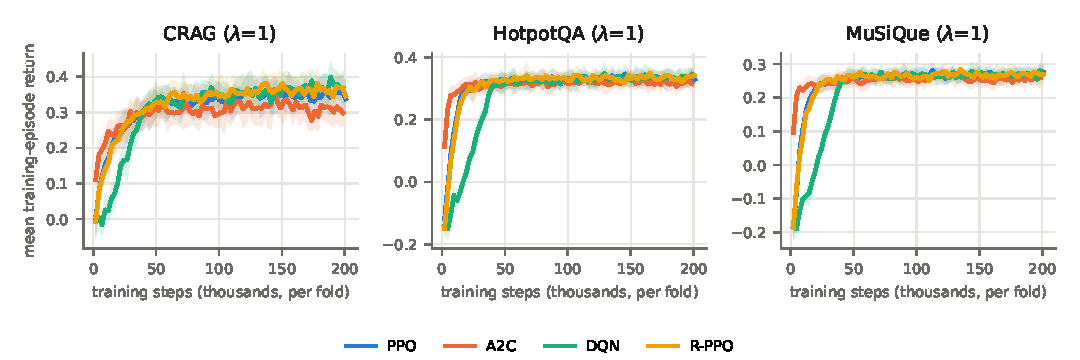
\includegraphics[width=0.92\linewidth]{figs/algorithms.pdf}
\caption{Training curves of MA+msg trained with four RL algorithms ($\lambda=1$; mean training-episode return, mean $\pm$ sd over seeds and folds).}
\label{fig:algorithms}
\Description{Three panels of mean training-episode return versus training steps for MA-Chunk trained with PPO, A2C, DQN and Recurrent PPO.}
\end{figure*}

\section{Abstention agent}\label{app:gate}

\begin{table}[t]
\centering\small
\caption{CRAG score without and with an abstention agent trained from the end-task reward (out-of-fold; seed 0). Abst.: abstention rate of the PPO gate.}
\label{tab:gate}
\setlength{\tabcolsep}{3pt}
\begin{tabular}{ll c cc c}
\toprule
 & Selector & None & PPO gate & Threshold & Abst. \\
\midrule
\multirow{2}{*}{CRAG}
 & MA+msg, $\lambda$=0.3 & $-$0.012 & 0.051 & \textbf{0.127} & 51\% \\
 & RRF top-3 & 0.068 & 0.041 & \textbf{0.142} & 37\% \\
\midrule
\multirow{5}{*}{HotpotQA}
 & MA, $\lambda$=0.3 & 0.154 & \textbf{0.172} & 0.169 & 24\% \\
 & MA+msg, $\lambda$=1.0 & 0.164 & 0.164 & 0.155 & 21\% \\
 & Single, $\lambda$=1.0 & 0.135 & 0.156 & 0.128 & 23\% \\
 & CE top-2 & 0.127 & 0.154 & 0.127 & 27\% \\
 & RRF top-3 & 0.113 & 0.145 & 0.130 & 28\% \\
\midrule
\multirow{3}{*}{MuSiQue}
 & MA+msg, $\lambda$=1.0 & $-$0.229 & \textbf{0.003} & $-$0.065 & 93\% \\
 & Single, $\lambda$=1.0 & $-$0.227 & $-$0.004 & $-$0.066 & 93\% \\
 & CE top-2 & $-$0.251 & $-$0.002 & $-$0.061 & 100\% \\
\bottomrule
\end{tabular}
\end{table}

\end{document}
